\documentclass{beamer}


\usepackage{amsmath}
\usepackage[style=alphabetic,url=true]{biblatex}
\usepackage{environ}
\usepackage{geometry}
\usepackage{graphicx}
\usepackage{tikz}
\usepackage[T2A]{fontenc}
\usepackage[utf8]{inputenc}
\usepackage[cache=false]{minted}
\usepackage{amsmath}
\usepackage{amsfonts}
\usepackage{amssymb}
\usepackage{calrsfs}


% \usetheme{Bergen}

\usecolortheme{beaver}

\setbeamertemplate{itemize item}[circle]
\setbeamertemplate{itemize subitem}{--}
\addtobeamertemplate{navigation symbols}{}{
  \usebeamerfont{footline}%
  \usebeamercolor[fg]{footline}%
  \hspace{1em}%
  \insertframenumber/\inserttotalframenumber
}
\graphicspath{ {./graphics/} }
\setminted[Python]{
  fontsize=\tiny
}
\BeforeBeginEnvironment{minted}{\medskip}
\AfterEndEnvironment{minted}{\medskip}



\title{
  Біткоїн та криптовалютні технології \\
  Лекція 4: Модель даних Біткоїна
}

\author{Юрій Жикін}
\date{29 вересня, 2022}

\begin{document}

\frame{\titlepage}

\begin{frame}
  \frametitle{Біткоїн-мережа}
  \begin{itemize}
  \item Біткоїн-мережа - це комп'ютерна мережа, що забезпечує у кожного учасника
    однакову копію бази даних з транзакціями, яка має спеціальну структуру
    (ланцюг блоків).
  \item ``Однакова копія'' означає, що у кожного учасника однаковий порядок 
    записів про транзакції.
  \end{itemize}
  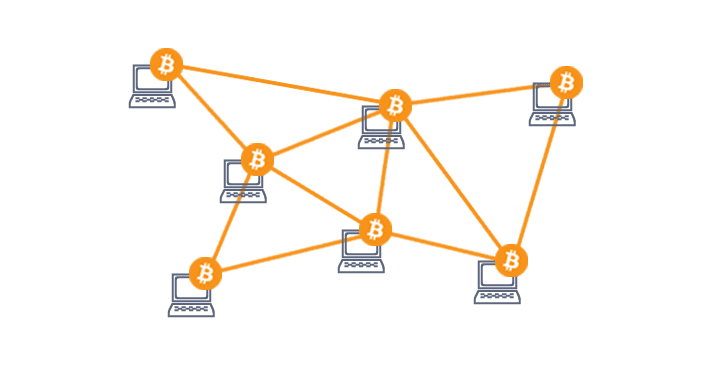
\includegraphics[width=\textwidth]{network}
\end{frame}

\begin{frame}
  \frametitle{Модель даних Біткоїна}
  \begin{itemize}
  \item \textbf{Ланцюг блоків} (або \textbf{часовий ланцюг}) - це розподілена,
    високо надлишкова база даних з транзакціями, що надійно гарантує
    \textit{існування, правильність і порядок} транзакцій.
  \item \textbf{Біткоїн-протокол} - це розподілений протокол, що підтримує базу
    даних Біткоїн-транзакцій і накладає чіткі вимоги щодо правильності
    транзакцій, а також надає гарантії безпеки бази даних через систему \textbf{``доказу
    виконаної роботи''} (\textbf{Proof-of-Work}).
  \item Якщо запис про транзакцію потрапив до бази даних, ми можемо бути впевнені,
    що транзакція
    \begin{itemize}
    \item точно відбулась,
    \item є гарантовано правильною,
    \item строго слідує чи передує іншим транзакціям.
    \end{itemize}
  \end{itemize}
\end{frame}

\begin{frame}
  \frametitle{Біткоїн-транзакції}
  \begin{itemize}
  \item Біткоїн-транзакція - це запис у базі даних, яку підтримує
    Біткоїн-мережа, про те, від кого, кому і скільки переказано біткоїнів.
  \end{itemize}
  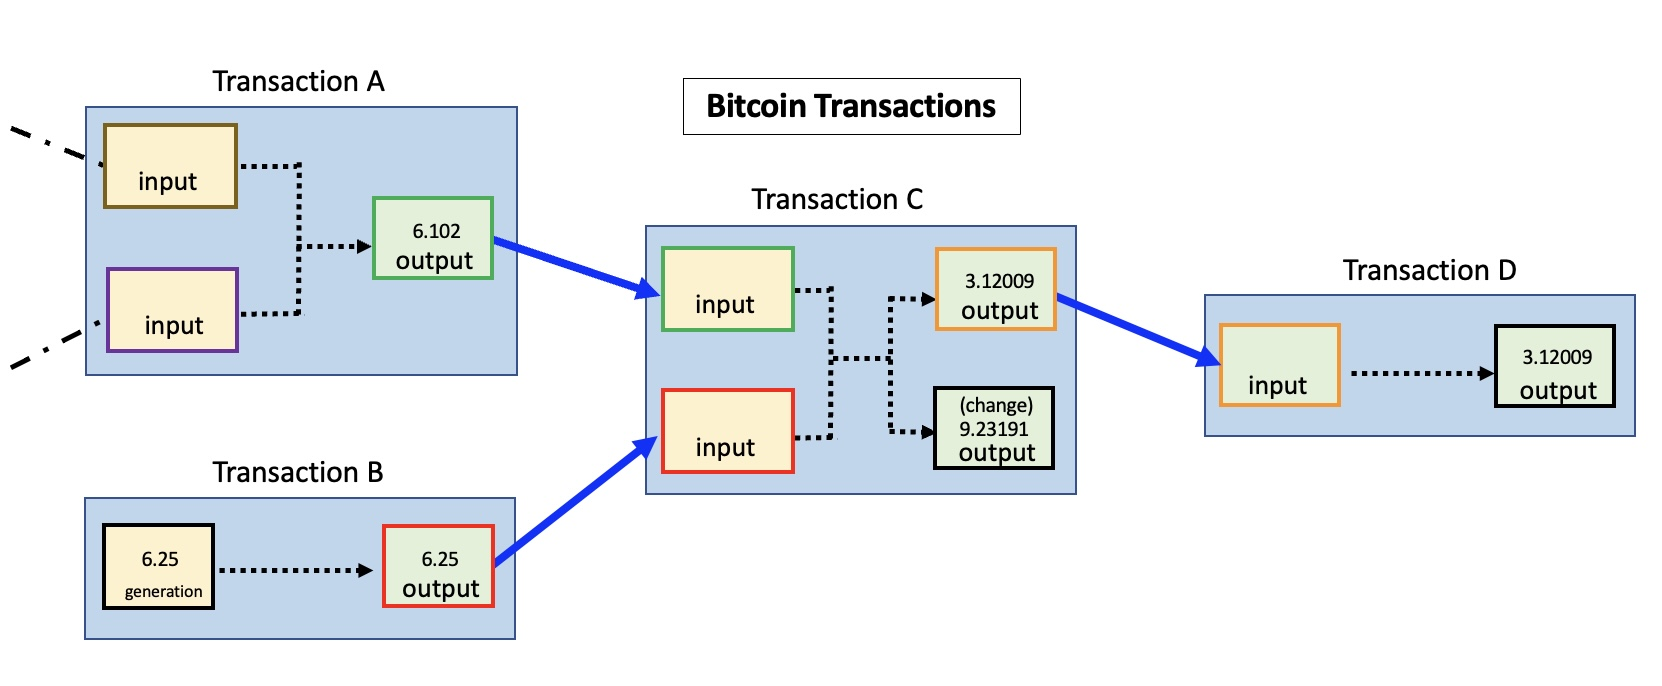
\includegraphics[width=\textwidth]{tx}
\end{frame}

\begin{frame}
  \frametitle{Транзакція}
  \begin{itemize}
  \item \textbf{Транзакція}
    \begin{itemize}
    \item \textbf{версія}
    \item \textbf{входи}
    \item \textbf{виходи}
    \item \textbf{``свідки''}
    \item \textbf{час блокування}
    \end{itemize}
  \item \textbf{Входи} - список транзакційних входів - посилання на виходи інших
    транзакцій, які ``знищуються'' даною транзакцією.
  \item \textbf{Виходи} - список щойно створених виходів, які вказують, куди
    переводяться всі біткоїни з виходів, на які посилаються входи.
  \item \textbf{Час блокування} накладає обмеження на момент у часі, коли
    транзакція може бути включена в базу даних.
  \end{itemize}
\end{frame}

\begin{frame}[fragile]
  \frametitle{Ідентифікатор транзакції}
  \begin{itemize}
  \item \textbf{Ідентифікатор траназкції} не є частиною структури транзакції,
    натомість він обчислюється з бінарного представлення самої транзакції:
    $$TXID = SHA256(SHA256(TX_{binary})$$
  \item $TXID$ - це послідовність з 32-х байтів, яка зазвичай представляється як
    64-символьний рядок у 16-му кодуванні:
    \begin{minted}{Python}
      169e1e83e930853391bc6f35f605c6754cfead57cf8387639d3b4096c54f18f4
    \end{minted}
  \end{itemize}
\end{frame}

\begin{frame}
  \frametitle{Транзакційний вихід}
  \begin{itemize}
  \item \textbf{Вихід}
    \begin{itemize}
    \item \textbf{кількість}
    \item \textbf{програма блокування}
    \end{itemize}
  \item \textbf{Кількість} - це кількість біткоїнів у даному виході, подана як
    ціле число, що означає кількість найменших одиниць, на які поділяється
    біткоїн, ``сатоші'' (1 BTC = $10^8$ сатоші).
  \item \textbf{Програма блокування} - обчислювальна задача (зазвичай ``надай
    правильний цифровий підпис''), яка повинна бути вирішена для того, щоб мати
    змогу використати даний вихід.
  \end{itemize}
\end{frame}

\begin{frame}
  \frametitle{Транзакційний вхід}
  \begin{itemize}
  \item \textbf{Вхід}
    \begin{itemize}
    \item \textbf{ідентифікатор попередньої транзакції}
    \item \textbf{індекс виходу у попередній транзакції}
    \item \textbf{програма розблокування}
    \end{itemize}
  \item Транзакційний вхід - це посилання на транзакційний вихід, який
    ``знищується'' у даній транзакції, а також програма розблокування.
  \item \textbf{Ідентифікатор попередньої транзакції} - TXID транзакції, що
    створила вихід.
  \item \textbf{Індекс у попередній транзакції} (\textbf{VOUT}) - індекс виходу
    у списку виходів в попередній транзакції.
  \item \textbf{Програма розблокування} - рішення задачі, сформульованої у
    програмі блокування цього виходу, предсталене, як програма мовою Bitcoin
    Script.
  \end{itemize}
\end{frame}

\begin{frame}
  \frametitle{Транзакційний ``свідок''}
  \begin{itemize}
  \item \textbf{Свідок} - це додаткова структура в Біткоїн-транзакції, яка була
    впроваджена у зміні до протоколу під назвою ``Відділений свідок'' (англ. \textbf{SegWit} -
    \textbf{Seg}regated \textbf{Wit}ness) 2017 року, як перший крок у
    довготривалому плані щодо вдосконалення безпеки, пропускної здатності та
    гнучкості Біткоїна.
  \item \textbf{Свідок} дозволяє зберігати складні \textit{скрипти розблокування}
    (рішення для \textit{скриптів блокування}, які складають значну частину всіх
    даних у транзакції.
  \end{itemize}
\end{frame}

\begin{frame}
  \frametitle{UTXO - Множина невикористаних транзакційних виходів}
  \begin{itemize}
  \item Всі біткоїни, які існують у системі, представлені так званою
    \textbf{множиною невикористаних транзакційних виходів} (\textbf{UTXOs}) -
    множинаю записів $(кількість, власник)$, які не були використані як входи у
    жодній іншій транзакції, і це можна довести.
  \item Кожна звичайна Біткоїн-транзакція знищує певну кількість існуючих UTXO і
    створює певну кількість нових UTXO.
  \item Ми кажемо, що певна сутність ``має'' біткоїн, якщо множина UTXO містить
    виходи, у яких частина $власник$ (\textbf{програма блокування}) якимось
    чином посилається на цю сутність.
  \end{itemize}
\end{frame}

\begin{frame}[fragile]
  \frametitle{Комісія за транзакцію}
  \begin{itemize}
  \item \textbf{Комісія за транзакцію} - це різниця між сумарною кількість
    біткоїнів у виходах, що знищуються цією транзакцією, та сумарною кількістю
    біткоїнів у виходах, що створюються цією транзакцією:
    $$TxFee = \sum_{i=1}^n InputAmount(txin_i) - \sum_{j=1}^m Amount(txout_j),$$
  \end{itemize}
\end{frame}

\begin{frame}
  \frametitle{Блок}
  \begin{itemize}
  \item \textbf{Блок}
    \begin{itemize}
    \item \textbf{заголовок}
    \item \textbf{транзакції}
    \end{itemize}
  \item \textbf{Заголовок} - це структура, що містить метадані про блок і всі
    компоненти, необхідні для роботи системи ``доказу виконаної роботи''.
  \item \textbf{Транзакції} - це впорядкований список транзакцій, що входять у
    даний блок.
  \end{itemize}
\end{frame}

\begin{frame}
  \frametitle{Заголовок блока 1/4}
  \begin{itemize}
  \item \textbf{Заголовок}
    \begin{itemize}
    \item \textbf{версія}
    \item \textbf{ідентифікатор попереднього блока}
    \item \textbf{корінь мерклевого дерева транзакції}
    \item \textbf{час створення блока}
    \item \textbf{задача ``доказу виконаної роботи''}
    \item \textbf{одноразовий ключ ``доказу виконаної роботи''}
    \end{itemize}
  \item \textbf{Ідентифікатор блока} (або \textbf{хеш блока}) обчислюється
    аналогічно до ідентифікатора транзакції:
    $$BlockID = SHA256(SHA256(BlockHeader_{binary}))$$
  \item \textbf{Ідентифікатор попереднього блока} - це компонент, що забезпечує
    утворення ``ланцюга'' з блоків (звідки й термін ``ланцюг блоків''
    (англ. blockchain): кожен наступний блок посилається на попередній блок, і
    зміна будь-якої інформації в будь-якому блоці змінює хеш даного блока, а
    також \textbf{хеші всіх блоків, що слідують за ним} завдяки лавинній
    властивості криптографічних хеш-функцій.
  \end{itemize}
\end{frame}

\begin{frame}
  \frametitle{Заголовок блока 2/4}
  \begin{itemize}
  \item \textbf{задача ``доказу виконаної роботи''} - це спеціальним чином
    закодоване число, яке є ціллю алгоритму ``доказу виконаної роботи'':
    ідентифікатор (хеш) блока повинен бути мешним за це число:
    $$ BlockID = SHA256(SHA256(BlockHeader)) < Target$$
  \item \textbf{Задача} переобчислюється кожних 2016 блоків (приблизно 2 тижні)
    для того, щоб підлаштувати складність знаходження рішень для нових блоків
    під вимогу, що середній період між блоками на кожному проміжку у 2016 блоків
    має становити 600 секунд (10 хвилин).
  \item Переобчислення значення задачі називається \textbf{коригуванням
      складності}: якщо середній час за останній 2016 блоків менший за 10
    хвилин, потрібно збільшити складність, обравши менше число-ціль, і навпаки.
  \item \textbf{Одноразовий ключ} (англ. \textbf{nonce} = \textbf{N}umber used
    \textbf{ONCE} - число, що використовується один раз) - значення, яке
    перебирається під час пошуку рішення алгоритму ``доказу виконаної роботи''
    для того щоб випадковим чином ``вгадати'' рішення.
  \end{itemize}
\end{frame}

\begin{frame}
  \frametitle{Заголовок блока 3/4}
  \begin{itemize}
  \item \textbf{Корінь мерклевого дерева транзакцій} - корінь мерклевого дерева
    - 32-байтна послідовність, яка криптографічно містить всі транзакції в
    даному блоці і фіксує їх порядок:
  \end{itemize}
  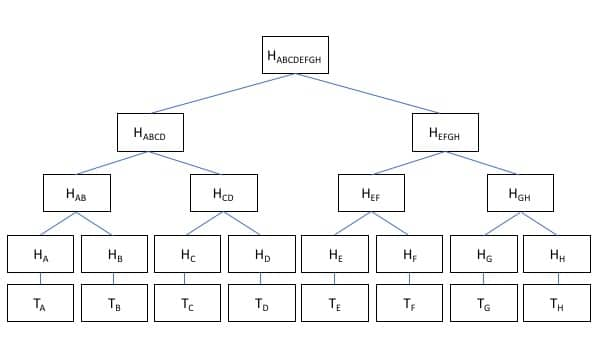
\includegraphics[width=\textwidth]{merkletree}
\end{frame}

\begin{frame}
  \frametitle{Заголовок блока 4/4}
  \begin{itemize}
  \item Ідентифікатори попередніх блоків зв'язують блоки та транзакції, що в них
    містяться, у лінійну послідовність завдяки криптографічним ``зобов'язанням''.
  \item Зміна лише одного біта в будь-якій транзакції повністю змінює корінь
    мерклевого дерева, що змінює ідентифікатор блока, що в свою чергу змінює
    ідентифікатор наступного блока, і так далі.
  \end{itemize}
  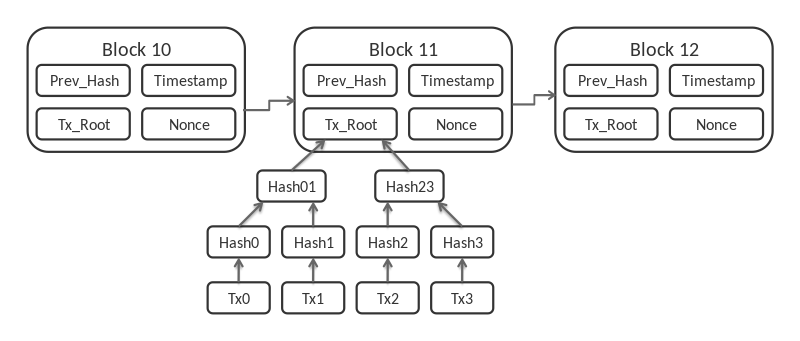
\includegraphics[width=\textwidth]{block-chain}
\end{frame}

\begin{frame}
  \frametitle{Майнінг}
  \begin{itemize}
  \item \textbf{Майнінг} (з англ. ``видобування'' блоків) - це процес обчислення
    рішення задачі ``доказу виконаної роботи'' для нових блоків.
  \item Майнер
    \begin{itemize}
    \item обирає певну кількість транзакцій з множини непідтверджених транзакцій,
    \item будує Мерклеве дерево і використовує корінь цього дерева та хеш
      попереднього (``найвищого'') відомого йому блока у заголовку нового блока.
    \item здійснює пошук шляхом ``грубої сили'' (повний перебір варіантів)
      рішення ``доказу виконаної роботи''
      $$SHA256(SHA256(BlockHeader)) < Target$$
    \item якщо рішення знайдено до того, як майнер дізнається, що хтось інший
      знайшов його раніше (отримає блок, що має той же блок як попередній),
      він публікує новий блок у мережу і сподівається, що він буде прийнятий, як
      новий найвищий блок.
    \end{itemize}
  \end{itemize}
\end{frame}

\begin{frame}
  \frametitle{Генеруюча транзакція і події поділу}
  \begin{itemize}
  \item Для того, щоб залучити майнерів до роботи на мережу, Біткоїн-протокол
    дозволяє їм додати першою транзакцією у блоці спеціальну транзакцію.
  \item Ця транзакція називається \textbf{генеруючою транзакцією}
    (англ. \textbf{coinbase}) і не має входів, лише виходи, кількість біткоїнів
    у яких встановлена протоколом, таким чином генеруючи нові біткоїни ``з
    повітря''.
  \item Окрім цього, майнер має право додати до нових біткоїнів сумарну різницю
    між входами та виходами всіх транзакцій у блоці (\textit{комісію за транзакції}).
  \item \textbf{Подія поділу навпіл} - для того, щоб гарантувати обмежену
    кількість біткоїнів в системі, кількість нових біткоїнів, що генеруються у
    блоці, почалась з 50 біткоїнів, зменшується вдвічі кожних 210000 блоків
    (приблизно кожних 4 роки), і рано чи пізно досягне 0 (орієнтовно через 120
    років), після чого кількість біткоїнів у системі перестане збільшуватись.
  \end{itemize}
\end{frame}

\begin{frame}
  \frametitle{Корисні ресурси}
  \begin{itemize}
  \item Learn me a Bitcoin by Greg Walker - ресурс, що містить багато цікавої
    інформації про технічні деталі роботи Біткоїн-протоколу
    \begin{itemize}
    \item https://learnmeabitcoin.com/
    \end{itemize}
  \end{itemize}
\end{frame}

\begin{frame}
  \frametitle{Кінець}
  \begin{center}
    Дякую за увагу!
  \end{center}
\end{frame}

\end{document}

%%% Local Variables:
%%% mode: latex
%%% TeX-master: t
%%% End:
